\documentclass{article}
\usepackage{graphicx}

\begin{document}
\section{Question 1}
\setcounter{subsection}{2}
\subsection{}
Time (in seconds) to complete standard training: 1359.3467. \\
Time (in seconds) to complete free adversarial training: 372.3792.
\subsection{}
\begin{center}
\begin{tabular}{||c c c||} 
    \hline
    Model/Task & Accuracy & PGD Success rate \\ [0.5ex] 
    \hline\hline
    Standard & 0.9170 & 0.8928 \\ 
    \hline
    Adv.-trained & 0.8087 & 0.3763 \\
    \hline 
\end{tabular}
\end{center}
Adversarial training significantly decreases the PGD succees rate, i.e increases robustness with the price of a small decrease in accuracy.
\subsection{}
\begin{center}
\begin{tabular}{||c c c c||} 
    \hline
    m/metric & Time & Accuracy & PGD Success rate \\ [0.5ex] 
    \hline\hline
    4 & 426.3014 & 0.8083 & 0.3790 \\ 
    \hline
    5 & 351.1917 & 0.7847 & 0.3868 \\
    \hline
    6 & 290.3951 & 0.7682 & 0.3953 \\
    \hline
    7 & 268.9399 & 0.7483 & 0.4095 \\
    \hline 
\end{tabular}
\end{center}
It seems that both the benign accuracy, robustness and training time decrease as m increases.
\section{Question 2}
\setcounter{subsection}{1}
\subsection{}
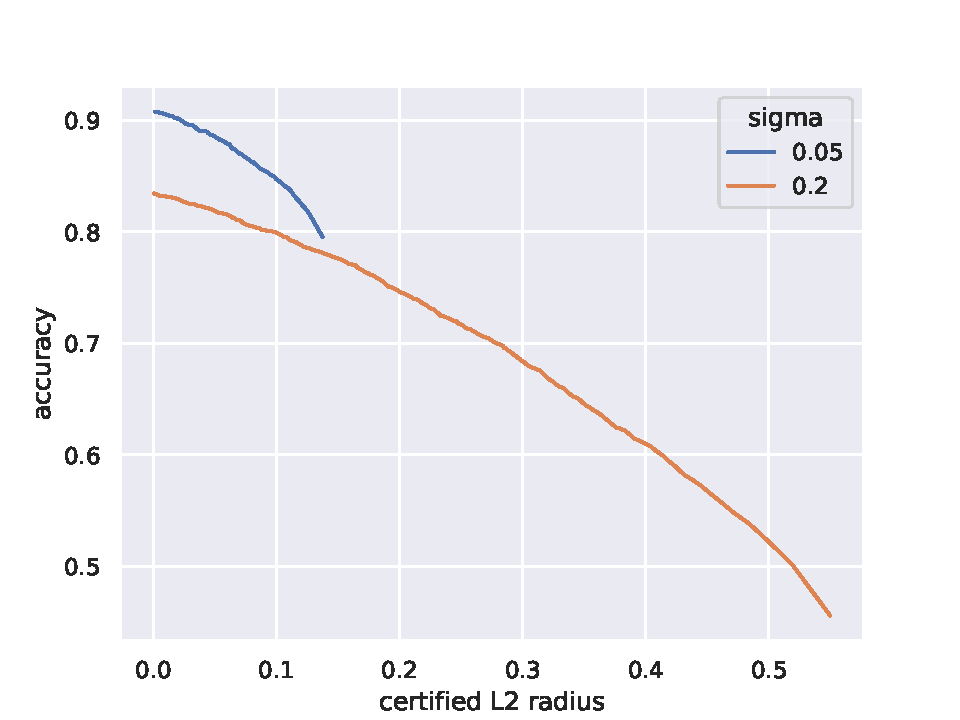
\includegraphics[scale=0.7]{randomized-smoothing-acc-vs-radius.pdf}

\section{Question 3}
\setcounter{subsection}{1}
\subsection{}
Model 1 is backdoored, the backdoor forces it to output class 0.
\subsection{}
\subsubsection{}
mask: \\

\includegraphics[scale=2]{backdoor-mask.jpg} \\
trigger: \\

\includegraphics[scale=2]{backdoor-trigger.jpg}
\subsubsection{}
Yes. The accuracy of Model 1 is only very slightly lower than that of Model 2 (0.9107 vs 0.9168).
\subsubsection{}
Very successful, its success rate is 0.9978.
\end{document}

